\documentclass[english]{article}

\usepackage{babel}
\usepackage{graphicx}
\usepackage{times}
\usepackage{pifont}
\usepackage[margin=1in]{geometry}
\usepackage{eurosym}
\usepackage{fancyhdr}
\usepackage[hidelinks]{hyperref}
\usepackage{float}
\usepackage{listings}

\pagestyle{fancy}
\fancyhf{}


%HEADER
%**************************************************************************************
\pagestyle{fancy}
\fancyhf{}
%**************************************************************************************
\lhead{Programming Serial Ports}		 	 
\rhead{Basics of Microprocessor technology} 
\lfoot{EFA12SF}
\cfoot{\thepage}
\rfoot{Nikolay Arsenov\\Alexey Tukalo}
%**************************************************************************************

\date{}
\setlength\parindent{0pt}

\begin{document}

\title{\vspace{2in}Programming Serial Ports\\
\small for Basics of Microprocessor technology\\
\vspace{0.5in}
\includegraphics{savonia.jpg}}

\nopagebreak
\maketitle


\vspace{3in}

\author{
\begin{flushright}
Nikolay Arsenov, Alexey Tukalo,\\
EFA12SF,\\
Information Technology,\\
Savonia University of Applied Sciences
\end{flushright}
}

\date{\today}
\thispagestyle{empty}

\newpage
\setcounter{page}{1}
\setcounter{tocdepth}{2}
\tableofcontents

\newpage

%MAIN CONTENT ******************************************************************************************************************

\section{Utilizing the serial communication}
Serial communication in such fields like telecommunication and computer science, is the process of sending data one unit per a time over a communication channel, bus or cable. In embedded systems, the AVR microcontrollers, serial communication also founded in UART to send digital signal from the microcontroller to a PC or otherwise, depends on what is our target. UART is a Universal Asynchronous Receiver/Transmitter. Transmitter (TX) is a device which sends data and Receiver (RX) gets the data from the transmitter. Transmitter and Receiver have flags to detect errors while transmission or receiving the frame, the same we can see in Network, for example in TCP/IP protocols, where each frame with our data transfers to the another device and in the frame there is also information about the state of connection, is there errors or loss and etc. If yes, send again, else, everything is good, wait a new packet with a frame.

\section{The features of USART circuit}
\begin{itemize}
\item Full Duplex Operation (Independent Serial Receive and Transmit Registers)
\item Asynchronous or Synchronous Operation
\item Master or Slave Clocked Synchronous Operation
\item High Resolution Baud Rate Generator
\item Supports Serial Frames with 5, 6, 7, 8, or 9 Data Bits and 1 or 2 Stop Bits
\item Odd or Even Parity Generation and Parity Check Supported by Hardware
\item Data OverRun Detection
\item Framing Error Detection
\item Noise Filtering Includes False Start Bit Detection and Digital Low Pass Filter
\item Three Separate Interrupts on TX Complete, TX Data Register Empty and RX Complete
\item Multi-processor Communication Mode
\item Double Speed Asynchronous Communication Mode
\end{itemize}
\section{Programming the transmission speed}
There are two different ways to set the necessary speed to the microcontroller, the first one is to calculate which value we should set to the UBRRnL and/or if we need UBRRnH. Or another way is to use the already calculated values from the “Boud Rate settings” Figure. We just need to know the frequency of our device, for example 16MHertz and what kind of speed (symbols per second or frames per second) we need.\\\\
For example, if we want to set our microcontroller speed equal to 9600 we can write this three lines:
\begin{lstlisting}
case 9600:UBRR0L=103; //speed 9600BD
		  UBRR0H=0;
\end{lstlisting}
For starting communication between transmitter and receiver, we have to set necessary flags to zero, set the Stop bit, Parity bit and Data Bits Format. Then enable transmitter and receiver:\\\\

UCSR0B=(1$<<$TXEN0) $\vee$ (1$<<$RXEN0);//enable transmitter and receiver.

\begin{figure}[H]
  \centering
  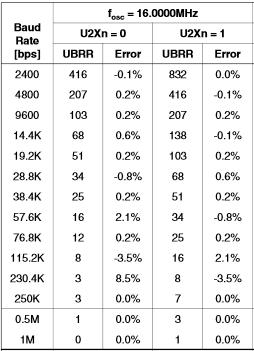
\includegraphics[scale=0.8]{MicroLab4/boundRate}
  \caption{ Boud Rate calculations} \label{tab:UCSZ} 
\end{figure}
\begin{figure}[H]
  \centering
  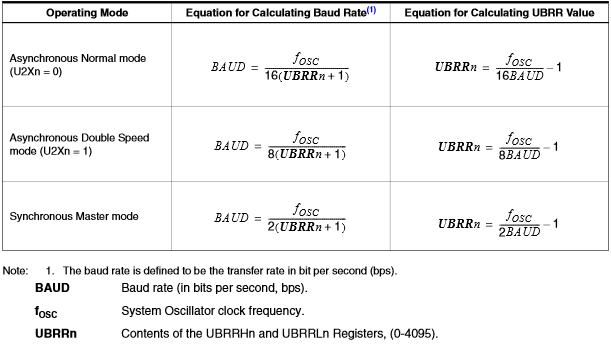
\includegraphics[scale=0.8]{MicroLab4/boundRateCalculations}
  \caption{Boud Rate settings} \label{tab:UCSZ} 
\end{figure}
\section{Programming the other serial parameters}
There are three main linear parameters of the frame format:
\begin{itemize}
\item Stop bit
\item Number of data bits
\item Parity settings
\end{itemize}
\subsection{Stop bit}
Stop bits are used to separate different frames, it can contain one or two bits. The settings should be made for transmitter, the receiver ignores it. The stop bits are controlled by USBSn register in according with table \ref{tab:USBS}.
\begin{figure}[H]
  \centering
  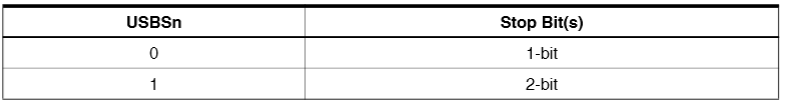
\includegraphics[scale=0.8]{MicroLab4/USBS}
  \caption{USBS Bit Settings} \label{tab:USBS} 
\end{figure}
\subsection{Number of data bits}
The number of data bits on the frame is controlled by UCSZn registers bits from 0 to 2. The settings have to be performed by table \ref{tab:UCSZ}.
\begin{figure}[H]
  \centering
  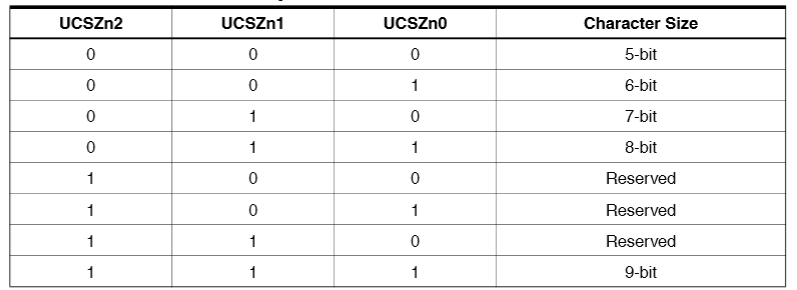
\includegraphics[scale=0.8]{MicroLab4/UCSZ}
  \caption{UCSZn Bits Setting} \label{tab:UCSZ} 
\end{figure}
\subsection{Parity settings}
Parity is some kind of error detection technique which is used in USART.
These bits enable and set type of parity generation and check. If enabled, the Transmitter will
automatically generate and send the parity of the transmitted data bits within each frame. The Receiver will generate a parity value for the incoming data and compare it to the UPMn setting. If a mismatch is detected, the UPEn Flag in UCSRnA will be set.
\begin{figure}[H]
  \centering
  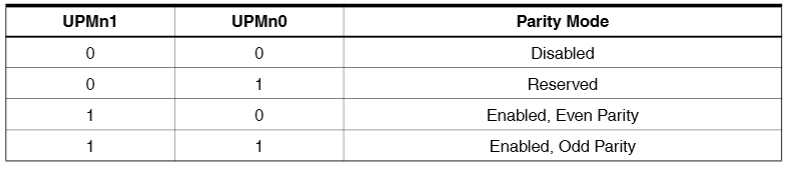
\includegraphics[scale=0.8]{MicroLab4/UPM}
  \caption{UPMn Bits Settings} 
\end{figure}
\section{The inspection of the data transmission}
The session between Transmitter and Receiver happens by sending frames one by one (frame – is a little piece of data). When the first portion taken, then sent and gotten by Receiver, UART starts new session with the same algorithms. \\\\
The Transmitter has two very important flags that indicate its state: USART Data Register Empty (UDREn) and Transmit Complete (TXCn). The Data Register Empty checks if the transmit buffer is ready to receive new data (empty or cleared), this bit sets and UCSRnA Register bit to zero. Then we enable Data Register Empty Interrupt Enable (UDRIEn) bit in UCSRnB, after that which will be executed. The Transmit Complete (TXCn) Flag bit is one, when entire frame in the Transmit Shift Register has been shifted out and there are no data in the buffer. The TXCn Flag bit is automatically cleared when transmit complete interrupt executed.\\\\
The Receiver has only one flag that indicated the Receiver state – the Receiver Complete (RXCn) Flag checks if there are unread data in the receiver buffer or not. If it exists – flag is one, and zero if the receiver buffer is empty. When the RXCn is set, there will be the Receive Complete Interrupt Enable (RXCIEn) in UCSRnB is set, the USART Receive Complete interrupt will be executed.\\\\
Errors checks on the USART Receiver, there are three Error Flags: Frame Error (FEn), Data OverRun (DORn) and Parity Error (UPEn). All can be accessed by reading UCSRnA.  All the flags located in the receive buffer together with the frame, which they indicate the error status. All flags must be set to zero when the UCSRnA is written for upward compatibility of future USART implementations. None of the Error Flags can generate interrupts.\\\\
The Frame Error (FEn) Flag indicates the state of the first stop bit of the next readable frame stored in the receive buffer. The FEn Flag is zero when the stop bit was correctly read (as one), and else if it was incorrect (zero). This flag can be used for detecting out-of-sync conditions, detecting break conditions and protocol handling. The FEn Flag is not affected by the setting of the USBSn bit in UCSRnC since the Receiver ignores all, except for the first, stop bits. \\\\
The Data OverRun (DORn) Flag indicates data loss due to a receiver buffer full condition. A Data OverRun occurs when the receive buffer is full (two characters), it is a new character waiting in the Receive Shift Register, and a new start bit is detected. If the DORn Flag is set there was one or more serial frame lost between the frame last read from UDRn, and the next frame read from UDRn. For compatibility with future devices, always write this bit to zero when writing to UCSRnA. The DORn Flag is cleared when the frame received was successfully moved from the Shift Register to the receive buffer. \\\\
The Parity Error (UPEn) Flag indicates that the next frame in the receive buffer had a Parity Error when received. If Parity Check is not enabled the UPEn bit will always be read zero. For compatibility with future devices, always set this bit to zero when writing to UCSRnA.
\section{Programming Tasks}

\subsection{The tasks from first to third}
\lstinputlisting[caption=L4\_123.c]{MicroLab4/L4_123.c}
\lstinputlisting[caption=L4\_123.h]{MicroLab4/L4_123.h}

\subsection{The fourth task}
\lstinputlisting[caption=L4\_4.c]{MicroLab4/L4_4.c}



\end{document}
